\documentclass[11pt]{article}
\usepackage[margin=0.78in]{geometry}
\usepackage{amsmath,amssymb}
\usepackage{booktabs}
\usepackage{graphicx}
\usepackage{xcolor}
\usepackage{hyperref}
\usepackage{tikz}
\usetikzlibrary{arrows.meta,positioning,shapes.geometric,fit,calc,matrix}
\hypersetup{colorlinks=true,linkcolor=blue!45!black,urlcolor=blue!55!black}
\setlength{\parindent}{0pt}
\setlength{\parskip}{0.55em}
\newcommand{\status}[1]{\textbf{Status: #1}}
\newcommand{\artifact}[1]{\texttt{\detokenize{#1}}}
\newcommand{\schematicnote}{\textit{This is a schematic, not evidence.}}
\newcommand{\lookat}{\textbf{What to look at.} }
\newcommand{\caveat}{\textbf{Caveat.} }
\newcommand{\bottomline}{\textbf{Bottom line.} }
\newcommand{\codeword}[1]{\texttt{#1}}
\definecolor{trusted}{HTML}{1B9E77}
\definecolor{broken}{HTML}{D73027}
\definecolor{caution}{HTML}{E6AB02}
\definecolor{muted}{HTML}{777777}
\definecolor{gpu}{HTML}{7570B3}

\title{Why the Repair Streams Native AMR Cells\\\large The one-off MPI+Kokkos reducer, without the abstraction tax}
\author{GOTHAM PDF reconstruction notes}
\date{June 2026}

\begin{document}
\maketitle
\status{Preferred calculation for additive PDFs. The original repair path is
strongly supported; the science catalog and complete Frontier run remain
unproven.}

\section{What we are trying to explain}

The task is to rebuild corrupted multidimensional PDFs from full-volume
\codeword{hydro\_w} AMR shards for five simulations and 161 snapshots. The
central design question is whether to construct a global dense cube first or
to reduce the native AMR cells directly.

The desired object is a weighted histogram. It is not a picture of a uniform
grid. That matters.

\section{The simple picture}

Read one bounded chunk of MeshBlocks. Compute the needed coordinates and
weights on the GPU. Add them into rank-local histograms. Throw the chunk away.
At the end, sum the histograms across MPI ranks.

The full snapshot never needs to coexist in memory. A dense Cartesian
intermediate would be enormous and would introduce interpolation choices that
can move mass or signed flux between bins.

\section{The cartoon version}

\begin{figure}[ht]
\centering
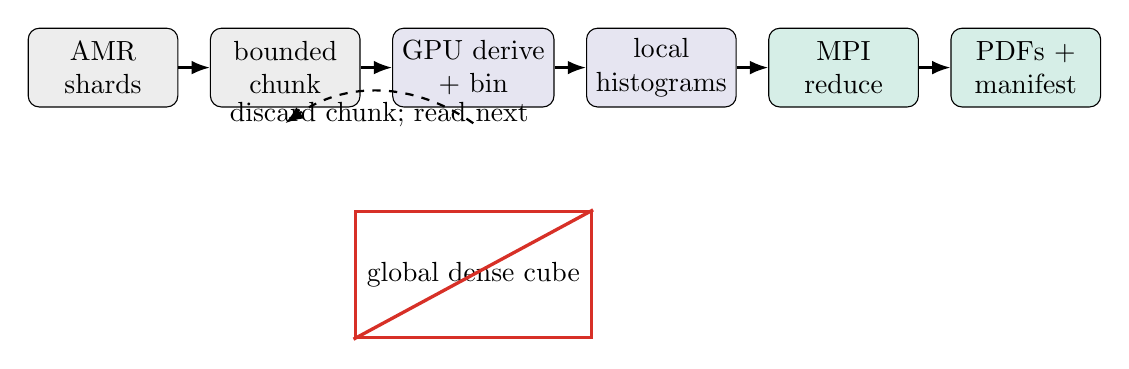
\begin{tikzpicture}[>=Latex,node distance=7mm and 4mm,
box/.style={draw,rounded corners,align=center,minimum height=10mm,minimum width=19mm},
io/.style={box,fill=black!7}, gpu/.style={box,fill=gpu!18},
ok/.style={box,fill=trusted!18}]
\node[io] (shards) {AMR\\shards};
\node[io,right=of shards] (pread) {bounded\\chunk};
\node[gpu,right=of pread] (derive) {GPU derive\\+ bin};
\node[gpu,right=of derive] (local) {local\\histograms};
\node[ok,right=of local] (reduce) {MPI\\reduce};
\node[ok,right=of reduce] (publish) {PDFs +\\manifest};
\draw[->,thick] (shards)--(pread);
\draw[->,thick] (pread)--(derive);
\draw[->,thick] (derive)--(local);
\draw[->,thick] (local)--(reduce);
\draw[->,thick] (reduce)--(publish);
\draw[->,thick,dashed] ($(derive.south)+(0,-2mm)$) to[bend right=35]
 node[below]{discard chunk; read next} ($(pread.south)+(0,-2mm)$);
\node[draw=broken,very thick,minimum width=30mm,minimum height=16mm,
below=13mm of derive] (dense) {global dense cube};
\draw[broken,very thick] (dense.south west)--(dense.north east);
\end{tikzpicture}
\caption{Each bounded AMR chunk contributes to persistent histograms and is
then discarded. At no point is a global dense cube assembled. \schematicnote}
\end{figure}

Follow the blue path left to right. The histograms survive each loop; the cell
chunk does not.

\section{The more precise version}

For product \(p\), bin \(b\), and AMR leaf cell \(c\),
\[
H_p(b)=\sum_{c\in\mathrm{leaves}}\Delta V_c\,w_p(q_c)\,
\mathbf{1}\!\left[B_p(x_c,q_c)=b\right].
\]
Here \(w_p\) is the pre-volume field: \(1\) for volume, density for mass, or a
flux density for transport products. The stored histogram is an integrated
weighted count, not a normalized probability density.
Each MPI rank accumulates \(H_p^{(r)}\), then
\[
H_p=\sum_r H_p^{(r)}.
\]
No global cell ordering is needed. The only non-negotiable condition is that
the accepted leaf set covers the domain exactly once:
\[
\sum_{c\in\mathrm{leaves}}\Delta V_c = V_{\mathrm{domain}},
\]
with no duplicate leaf and no ancestor counted alongside a descendant.
That is the mathematical requirement. The current implementation checks
contiguous shard identity, duplicate logical keys, ancestor/descendant pairs,
and summed volume. Those are strong necessary invariants, but they do not
prove arbitrary physical coverage: a hole and a distinct-key equal-volume
overlap could in principle compensate.

The useful memory claim is about field data, not every byte in the program.
A phase-wise peak estimate is
\[
M_{\rm peak}\simeq \max(M_{\rm process},M_{\rm validate},M_{\rm reduce}),
\]
\[
\begin{split}
M_{\rm process}&\simeq M_{\rm host\,chunk}+M_{\rm device\,chunk}
 + M_{\rm hist}+O(N_{{\rm blocks},r}),\\
M_{\rm validate,root}&=O(N_{\rm blocks,global}),\\
M_{\rm reduce,root}&\simeq 2M_{\rm hist}
 + \max_p(8N_{{\rm bins},p})+O(N_{\rm blocks,global}).
\end{split}
\]
There is one line worth noticing: the large field-data term follows the chunk
size, not the size of the full snapshot. Metadata and root reduction storage
still grow and must be measured at complete-snapshot scale.

One FP64 histogram uses \(0.292\) GiB for the original repair catalog and
\(0.325\) GiB for all 76 products. Those are not peak-memory measurements. The
dominant field-data memory follows
\codeword{--chunk-blocks}, not the full snapshot. Rank-zero key gathering,
product reductions, and output buffers still grow with the complete run and
must be measured on Frontier.

Now compare that with the tempting alternative. A uniform 8 pc representation
of a \(400\) kpc domain would contain roughly
\[
(400/0.008)^3=1.25\times10^{14}
\]
cells. Eight float32 fields alone would take about \(4\) PB decimal. That is
not merely inconvenient. It is the wrong intermediate for a histogram
reduction.

\section{What this idea predicts}

If direct AMR reduction is really the right calculation, it has to survive six
checks.

\begin{itemize}
  \item A separately implemented cell-by-cell oracle should match every emitted
        product under the stated physical conventions.
  \item Changing MPI rank count should not change the scientific result beyond
        floating-point reduction order.
  \item Products sharing the same weight should close to the same global total.
  \item The method should process real shards with bounded field-data memory.
  \item A deliberately partial run should work but must refuse to claim global
        AMR closure.
  \item A complete run should reject missing shards, duplicate logical keys,
        ancestor/descendant pairs, and wrong summed volume. Stronger geometry
        checks are needed to reject arbitrary physical holes or overlaps.
\end{itemize}

Here ``complete'' means that the job supplies the expected contiguous shard
count explicitly. The executable does not infer completeness merely because no
input limit was requested.

\section{What the evidence actually shows}

\begin{figure}[ht]
\centering
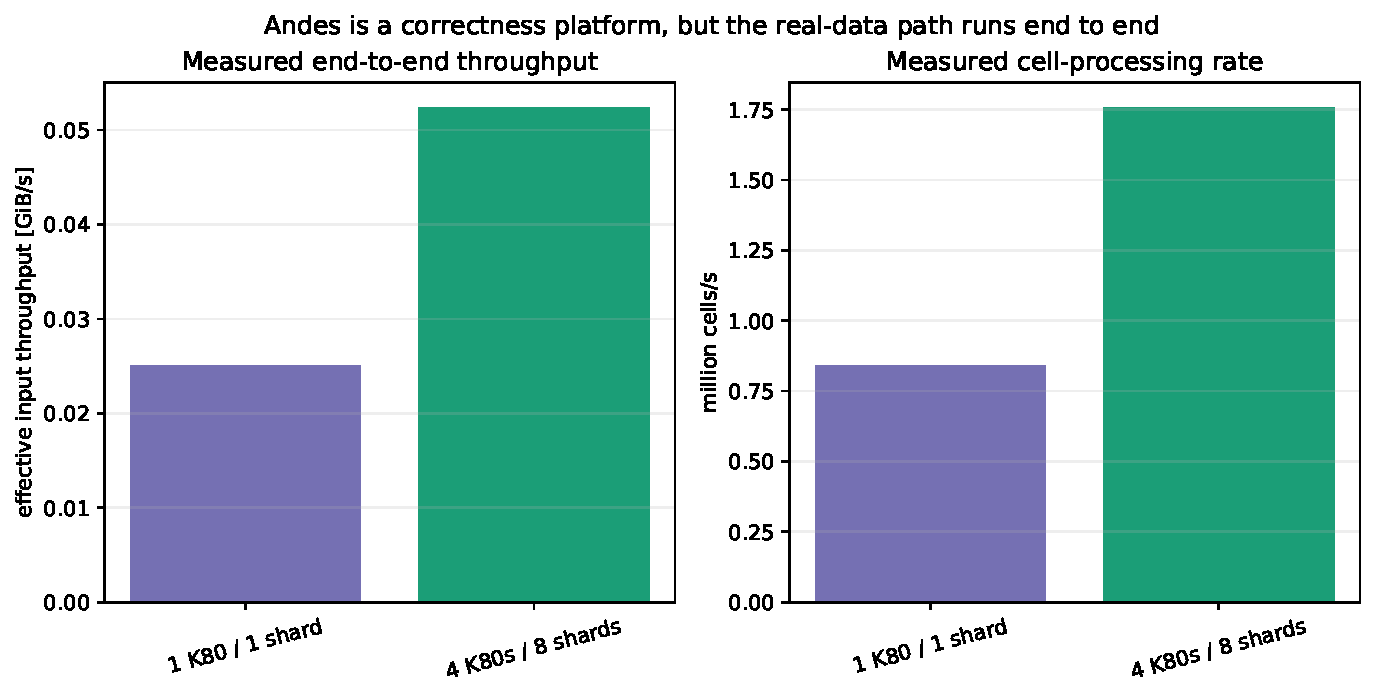
\includegraphics[width=0.96\linewidth]{figures/andes_runtime_throughput.pdf}
\caption{Measured end-to-end rates for one complete real shard on one K80 and
eight complete real shards on four K80 GPUs, both using the 14-product
\codeword{original} catalog. Exact logs are recorded in the evidence audit.}
\end{figure}

\lookat Look at the move from one K80 to four K80s. The job processes eight
times as much real data, but aggregate throughput improves by only about
\(2.09\times\). The useful result is not that K80 is fast. It is not. The
useful result is that the full real-data path runs end to end: fixed-record
input, device derivation, FP64 histogram accumulation, MPI reduction, and
publication. Four GPUs process 20.000 GiB and 671,088,640 cells successfully.

\caveat The aggregate four-K80 speedup is only about \(2.09\times\) relative
to the one-K80 rate. This tells us the real path executes, not that production
will be efficient. MI250X atomics, I/O overlap, root-memory growth, and
GPU-aware reduction still need profiling.

\begin{figure}[ht]
\centering
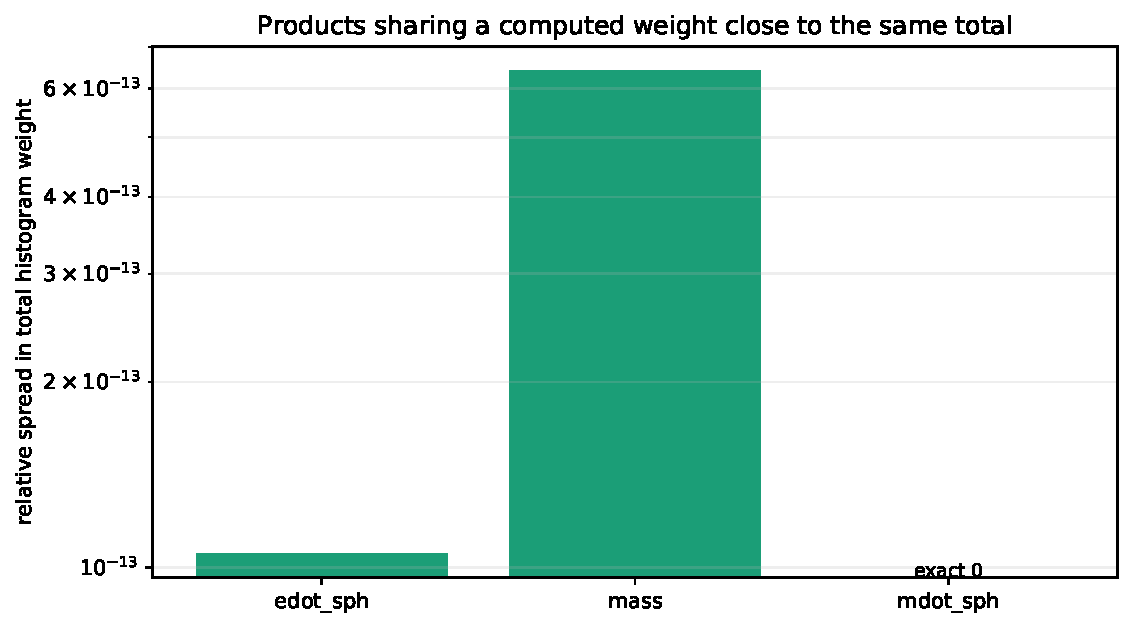
\includegraphics[width=0.82\linewidth]{figures/same_weight_total_closure.pdf}
\caption{Eight-shard products that use the same weight close to the same total.
This is a narrow deposit/reduction invariant, not an external validation of the
weight formula.}
\end{figure}

\lookat Look at how tightly the same-weight families cluster near zero spread.
Their relative differences are around \(10^{-13}\). Different axis choices
redistribute the same computed weight between bins without dropping deposits.
A shared wrong weight formula would still pass this test.

\section{The key figures}

These figures do different jobs. One says the pipeline runs. One says the
bookkeeping closes. The corruption document's archived controls ask the harder
question: did we reconstruct the right answer?

\section{What works}

The evidence comes in layers. The separate Python implementation checks the
agreed formulas. The
one-rank/two-rank tests check decomposition. The real-shard runs check the
actual I/O, GPU, MPI, and publication path. The archived controls then check
the original energy-flux repair path against surviving external evidence.

\begin{itemize}
  \item The separately implemented Python oracle covers 14/14 original
        products and 20/62 science products, plus boundary semantics, signed
        weights, and synthetic \(32^3\) and \(64^3\) block layouts.
  \item Synthetic one-rank and two-rank outputs agree.
  \item The production analysis reader accepts the dense reconstructed files.
  \item One block with all 76 products runs on GPU.
  \item One complete real shard and an eight-shard/four-GPU real run complete.
  \item The intact archived energy-flux controls agree closely.
  \item Publication is fail-closed only for consumers that require the final
        manifest; individual product files are renamed before that manifest.
\end{itemize}

\section{What does not work}

The current kernel is simple enough to audit, and simple enough to bottleneck.
Every cell loops over selected products and performs global FP64 atomics.
Reading, copying, and kernel work are serialized. MPI reduction is host-staged.
Those are plausible performance limits on Frontier.

They are not arguments for a dense cube. They are optimization questions
inside this reducer.

This reducer also cannot reconstruct quantities absent from
\codeword{hydro\_w}: magnetic diagnostics, particle history, ion fractions,
shock history, or event provenance. Cooling products were excluded because
the exact cooling, shielding, and potential reconstruction was not independently
validated.

The 62 science products are useful candidates, not externally validated truth.
Many use mass, volume, scalar, metal, dust, Mach, angular-momentum, or vertical
transport conventions that the surviving archived controls do not test.

\section{How this could be wrong}

The most serious failure would be a complete snapshot that passes current
global invariants but has a physical hole compensated by an equal-volume
overlap. The current path validates contiguous shard identity, complete
headers, unique leaf keys, ancestor/descendant exclusion, and domain-volume
closure. It still needs logical-key bounds and geometry-to-key consistency
checks before it can claim exact spatial coverage.

Another risk is semantic drift: ``improving'' legacy temperature, flux, or
underflow conventions would produce scientifically different PDFs. The
separate oracle pins the agreed definitions down, but it cannot rule out a
shared scientific misunderstanding.

\section{What would decide the issue}

One complete \codeword{res\_8pc/phase2/00028} Frontier reconstruction is the
next test that can still change our mind about scale. Before claiming exact
coverage, add a geometry/key consistency check and a malformed-mesh negative
test. Before promoting the science catalog, hand-check representative real
cells against independently stated physical conventions. Separate
\codeword{original}, \codeword{science}, and \codeword{all} runs then decide
whether the current atomic design is fast enough or needs targeted optimization.

\section{Bottom line}

\bottomline PDFs are additive reductions over AMR leaves. The streaming
MPI+Kokkos reducer performs that operation directly, with bounded field-data
memory and
without inventing a dense grid that the PDF calculation never needed. The
streaming architecture and original repair path are strongly supported. Exact
spatial-coverage validation, the broader science catalog, and MI250X
performance remain open.

\appendix
\section{Revision notes}
This document was revised after solution-advocate, logic/technical,
evidence/figure, red-team, visual-design, human-editor, and reproducibility
checks. Pass two separated architecture validation from science-product
validation, narrowed the memory claim, recast same-weight closure as an
internal checksum, and weakened exact-coverage and publication claims to match
the implementation. Review records live in the local \codeword{notes/}
directory.
\end{document}
